\documentclass{article}    
\usepackage[utf8]{inputenc}    
    
\title{Épisode 4}    
\author{Jean-Baptiste Bertrand}    
\date{\today}    
    
\setlength{\parskip}{1em}    
    
\usepackage{physics}    
\usepackage{graphicx}    
\usepackage{svg}    
\usepackage[utf8]{inputenc}    
\usepackage[T1]{fontenc}    
\usepackage[french]{babel}    
\usepackage{fancyhdr}    
\usepackage[total={19cm, 22cm}]{geometry}    
\usepackage{enumerate}    
\usepackage{enumitem}    
\usepackage{stmaryrd}    
\usepackage{mathtools,slashed}
%\usepackage{mathtools}
\usepackage{cancel}
    
\usepackage{pdfpages}
%packages pour faire des math    
%\usepackage{cancel} % hum... pas sur que je vais le garder mais rester que des fois c'est quand même sympatique...
\usepackage{amsmath, amsfonts, amsthm, amssymb}    
\usepackage{esint}  
\usepackage{dsfont}

\usepackage{import}
\usepackage{pdfpages}
\usepackage{transparent}
\usepackage{xcolor}
\usepackage{tcolorbox}

\usepackage{mathrsfs}
\usepackage{tensor}

\usepackage{tikz}
\usetikzlibrary{quantikz}
\usepackage{ upgreek }

\newcommand{\incfig}[2][1]{%
    \def\svgwidth{#1\columnwidth}
    \import{./figures/}{#2.pdf_tex}
}

\newcommand{\cols}[1]{
\begin{pmatrix}
	#1
\end{pmatrix}
}

\newcommand{\avg}[1]{\left\langle #1 \right\rangle}
\newcommand{\lambdabar}{{\mkern0.75mu\mathchar '26\mkern -9.75mu\lambda}}

\pdfsuppresswarningpagegroup=1

\begin{document}


\section*{2.4.7:} Calculer le transport parallèle d'un vecteur autour du cercle $u=u_0$ sur le cône $p(u,v) = \left( u\cos v,\, u\sin v,\, cu \right) $  

\begin{figure}[ht]
    \centering
    \incfig{cône}
    \caption{Cône}
    \label{fig:cône}
\end{figure}

\begin{tcolorbox}[title=Rappel]
	$f(t) p_u + g(t) p_v$ est $\|$ le long de $\alpha(t) = p(u(t),v(t))$ ssi
	$$\cols{f'\\ g'} = - \cols{u'\Gamma_{uu}^{u}+ v'\Gamma_{uv}^{u}& u'\Gamma_{uv}^{u} + v'\Gamma_{vv}^{u}\\u'\Gamma_{uu}^{v}+ v'\Gamma_{uv}^{v}& u'\Gamma_{uv}^{v}+ v'\Gamma_{vv}^v}\cols{f\\g}$$ 
\end{tcolorbox}

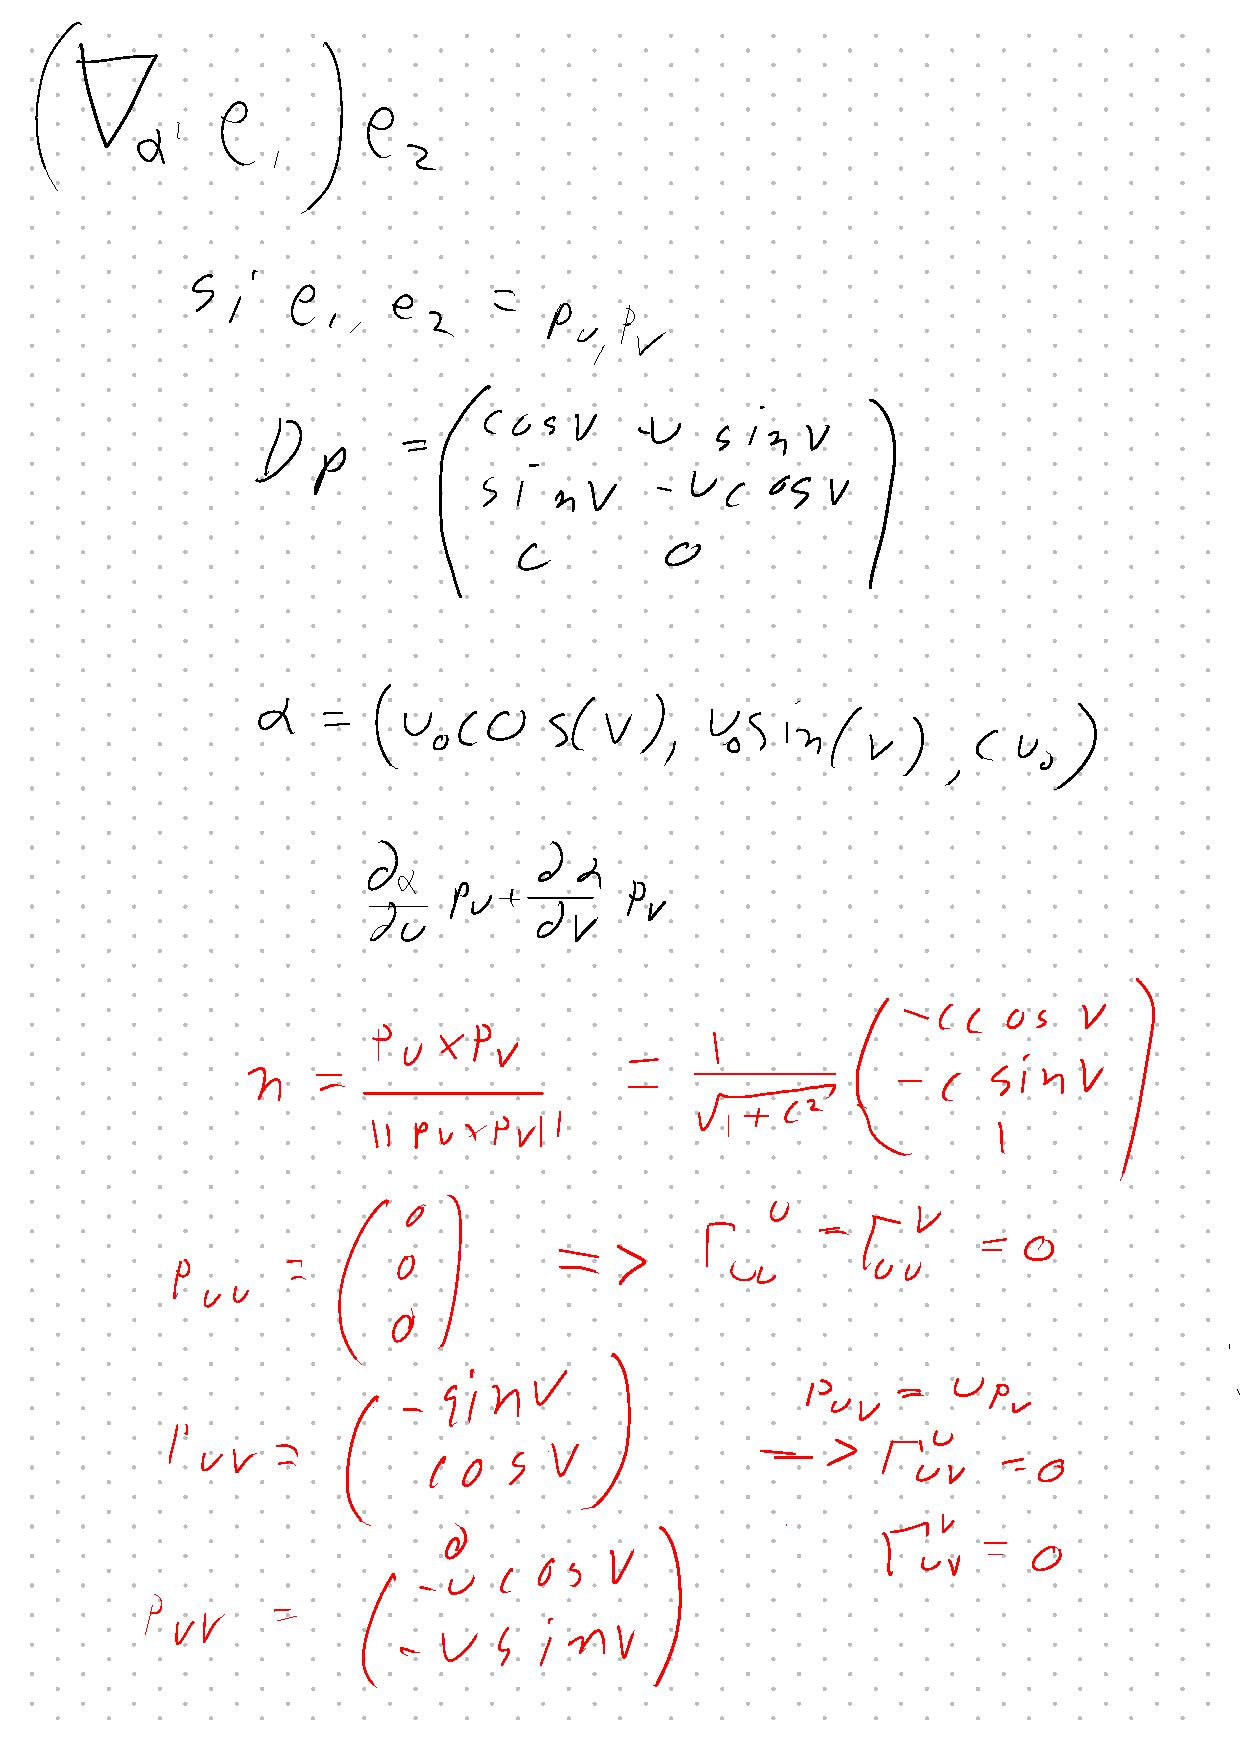
\includepdf[pages=-]{Exercices/2.4.7.pdf}


\begin{figure}[ht]
    \centering
    \incfig{isomorphisme-euclidien}
    \caption{Isomorphisme Euclidien}
    \label{fig:isomorphisme-euclidien}
\end{figure}


\section*{Exer}



\end{document}
